\ifx\allfiles\undefined
\documentclass[12pt, a4paper, oneside, UTF8]{ctexbook}
\def\path{../config}
\usepackage{amsmath}
\usepackage{amsthm}
\usepackage{array}
\usepackage{amssymb}
\usepackage{graphicx}
\usepackage{mathrsfs}
\usepackage{enumitem}
\usepackage{geometry}
\usepackage[colorlinks, linkcolor=black]{hyperref}
\usepackage{stackengine}
\usepackage{yhmath}
\usepackage{extarrows}
% \usepackage{unicode-math}
\usepackage{esint}
\usepackage{multirow}
\usepackage{fancyhdr}
\usepackage[dvipsnames, svgnames]{xcolor}
\usepackage{listings}
\usepackage{float} % Required for the H float option
\definecolor{mygreen}{rgb}{0,0.6,0}
\definecolor{mygray}{rgb}{0.5,0.5,0.5}
\definecolor{mymauve}{rgb}{0.58,0,0.82}
\definecolor{NavyBlue}{RGB}{0,0,128}
\definecolor{Rhodamine}{RGB}{255,0,255}
\definecolor{PineGreen}{RGB}{0,128,0}

\graphicspath{ {figures/},{../figures/}, {config/}, {../config/} }

\linespread{1.6}

\geometry{
    top=25.4mm, 
    bottom=25.4mm, 
    left=20mm, 
    right=20mm, 
    headheight=2.17cm, 
    headsep=4mm, 
    footskip=12mm
}

\setenumerate[1]{itemsep=5pt,partopsep=0pt,parsep=\parskip,topsep=5pt}
\setitemize[1]{itemsep=5pt,partopsep=0pt,parsep=\parskip,topsep=5pt}
\setdescription{itemsep=5pt,partopsep=0pt,parsep=\parskip,topsep=5pt}

\lstset{
    language=Mathematica,
    basicstyle=\tt,
    breaklines=true,
    keywordstyle=\bfseries\color{NavyBlue}, 
    emphstyle=\bfseries\color{Rhodamine},
    commentstyle=\itshape\color{black!50!white}, 
    stringstyle=\bfseries\color{PineGreen!90!black},
    columns=flexible,
    numbers=left,
    numberstyle=\footnotesize,
    frame=tb,
    breakatwhitespace=false,
} 

\lstset{
    language=TeX, % 设置语言为 TeX
    basicstyle=\ttfamily, % 使用等宽字体
    breaklines=true, % 自动换行
    keywordstyle=\bfseries\color{NavyBlue}, % 关键字样式
    emphstyle=\bfseries\color{Rhodamine}, % 强调样式
    commentstyle=\itshape\color{black!50!white}, % 注释样式
    stringstyle=\bfseries\color{PineGreen!90!black}, % 字符串样式
    columns=flexible, % 列的灵活性
    numbers=left, % 行号在左侧
    numberstyle=\footnotesize, % 行号字体大小
    frame=tb, % 顶部和底部边框
    breakatwhitespace=false % 不在空白处断行
}

% \begin{lstlisting}[language=TeX] ... \end{lstlisting}

% 定理环境设置
\usepackage[strict]{changepage} 
\usepackage{framed}

\definecolor{greenshade}{rgb}{0.90,1,0.92}
\definecolor{redshade}{rgb}{1.00,0.88,0.88}
\definecolor{brownshade}{rgb}{0.99,0.95,0.9}
\definecolor{lilacshade}{rgb}{0.95,0.93,0.98}
\definecolor{orangeshade}{rgb}{1.00,0.88,0.82}
\definecolor{lightblueshade}{rgb}{0.8,0.92,1}
\definecolor{purple}{rgb}{0.81,0.85,1}

\theoremstyle{definition}
\newtheorem{myDefn}{\indent Definition}[section]
\newtheorem{myLemma}{\indent Lemma}[section]
\newtheorem{myThm}[myLemma]{\indent Theorem}
\newtheorem{myCorollary}[myLemma]{\indent Corollary}
\newtheorem{myCriterion}[myLemma]{\indent Criterion}
\newtheorem*{myRemark}{\indent Remark}
\newtheorem{myProposition}{\indent Proposition}[section]

\newenvironment{formal}[2][]{%
	\def\FrameCommand{%
		\hspace{1pt}%
		{\color{#1}\vrule width 2pt}%
		{\color{#2}\vrule width 4pt}%
		\colorbox{#2}%
	}%
	\MakeFramed{\advance\hsize-\width\FrameRestore}%
	\noindent\hspace{-4.55pt}%
	\begin{adjustwidth}{}{7pt}\vspace{2pt}\vspace{2pt}}{%
		\vspace{2pt}\end{adjustwidth}\endMakeFramed%
}

\newenvironment{definition}{\vspace{-\baselineskip * 2 / 3}%
	\begin{formal}[Green]{greenshade}\vspace{-\baselineskip * 4 / 5}\begin{myDefn}}
	{\end{myDefn}\end{formal}\vspace{-\baselineskip * 2 / 3}}

\newenvironment{theorem}{\vspace{-\baselineskip * 2 / 3}%
	\begin{formal}[LightSkyBlue]{lightblueshade}\vspace{-\baselineskip * 4 / 5}\begin{myThm}}%
	{\end{myThm}\end{formal}\vspace{-\baselineskip * 2 / 3}}

\newenvironment{lemma}{\vspace{-\baselineskip * 2 / 3}%
	\begin{formal}[Plum]{lilacshade}\vspace{-\baselineskip * 4 / 5}\begin{myLemma}}%
	{\end{myLemma}\end{formal}\vspace{-\baselineskip * 2 / 3}}

\newenvironment{corollary}{\vspace{-\baselineskip * 2 / 3}%
	\begin{formal}[BurlyWood]{brownshade}\vspace{-\baselineskip * 4 / 5}\begin{myCorollary}}%
	{\end{myCorollary}\end{formal}\vspace{-\baselineskip * 2 / 3}}

\newenvironment{criterion}{\vspace{-\baselineskip * 2 / 3}%
	\begin{formal}[DarkOrange]{orangeshade}\vspace{-\baselineskip * 4 / 5}\begin{myCriterion}}%
	{\end{myCriterion}\end{formal}\vspace{-\baselineskip * 2 / 3}}
	

\newenvironment{remark}{\vspace{-\baselineskip * 2 / 3}%
	\begin{formal}[LightCoral]{redshade}\vspace{-\baselineskip * 4 / 5}\begin{myRemark}}%
	{\end{myRemark}\end{formal}\vspace{-\baselineskip * 2 / 3}}

\newenvironment{proposition}{\vspace{-\baselineskip * 2 / 3}%
	\begin{formal}[RoyalPurple]{purple}\vspace{-\baselineskip * 4 / 5}\begin{myProposition}}%
	{\end{myProposition}\end{formal}\vspace{-\baselineskip * 2 / 3}}


\newtheorem{example}{\indent \color{SeaGreen}{Example}}[section]
\renewcommand{\proofname}{\indent\textbf{\textcolor{TealBlue}{Proof}}}
\newenvironment{solution}{\begin{proof}[\indent\textbf{\textcolor{TealBlue}{Solution}}]}{\end{proof}}

% 自定义命令的文件

\def\d{\mathrm{d}}
\def\R{\mathbb{R}}
%\newcommand{\bs}[1]{\boldsymbol{#1}}
%\newcommand{\ora}[1]{\overrightarrow{#1}}
\newcommand{\myspace}[1]{\par\vspace{#1\baselineskip}}
\newcommand{\xrowht}[2][0]{\addstackgap[.5\dimexpr#2\relax]{\vphantom{#1}}}
\newenvironment{mycases}[1][1]{\linespread{#1} \selectfont \begin{cases}}{\end{cases}}
\newenvironment{myvmatrix}[1][1]{\linespread{#1} \selectfont \begin{vmatrix}}{\end{vmatrix}}
\newcommand{\tabincell}[2]{\begin{tabular}{@{}#1@{}}#2\end{tabular}}
\newcommand{\pll}{\kern 0.56em/\kern -0.8em /\kern 0.56em}
\newcommand{\dive}[1][F]{\mathrm{div}\;\boldsymbol{#1}}
\newcommand{\rotn}[1][A]{\mathrm{rot}\;\boldsymbol{#1}}

% 修改参数改变封面样式,0 默认原始封面、内置其他1、2、3种封面样式
\def\myIndex{0}


\ifnum\myIndex>0
    \input{\path/cover_package_\myIndex}
\fi

\def\myTitle{标题:一份LaTeX笔记模板}
\def\myAuthor{作者名称}
\def\myDateCover{封面日期: \today}
\def\myDateForeword{前言页显示日期: \today}
\def\myForeword{前言标题}
\def\myForewordText{
    
    这是一个基于\LaTeX{}的模板,用于撰写学习笔记。

    模板旨在提供一个简单、易用的框架,以便你能够专注于内容,而不是排版细节,如不是专业者,不建议使用者在模板细节上花费太多时间,而是直接使用模板进行笔记撰写。遇到问题,再进行调整解决。
}
\def\mySubheading{副标题}


\begin{document}
% \input{\path/cover_text_\myIndex.tex}

\newpage
\thispagestyle{empty}
\begin{center}
    \Huge\textbf{\myForeword}
\end{center}
\myForewordText
\begin{flushright}
    \begin{tabular}{c}
        \myDateForeword
    \end{tabular}
\end{flushright}

\newpage
\pagestyle{plain}
\setcounter{page}{1}
\pagenumbering{Roman}
\tableofcontents

\newpage
\pagenumbering{arabic}
\setcounter{chapter}{-1}
\setcounter{page}{1}

\pagestyle{fancy}
\fancyfoot[C]{\thepage}
\renewcommand{\headrulewidth}{0.4pt}
\renewcommand{\footrulewidth}{0pt}








\else
\fi

\chapter{地震作用}
地震按其产生的原因,可分为

\begin{itemize}
    \item  火山地震:火山活动(爆发或爆发前夕)引起
    \item 陷落地震:地下空洞(岩洞、矿井等)突然塌陷而引起
    \item 构造地震:地质运动引起(占世界地总数90\%以上,{\color{red}也是破坏力最大的})
\end{itemize}

地幔热对流是引起地质运动的最主要原因,其他原因包括地球的自转与公转、月球和太阳的引力影响等。
地质运动使地壳岩层变形而产生应力,岩层变形不断累积会使应力增大,当岩层应力大于岩石强度时,岩层会突然破裂,岩层破裂后将以震动的方式释放能量并产生地震波,地震波到达观测点地面引起地面运动,形成“地震”。

\textbf{地震术语:}

\begin{enumerate}
    \item 震源:即发震点,是指岩层断裂处
    \item 震中:指震源正上方的地面地点
    \item 震源深度:指震中至震源的距离
    \item 震中距:指地面某处到震中的距离
\end{enumerate}

\begin{remark}
震源深度:

浅源地震(h$\leq$60km)

中源地震(60km$\leq$h$\leq$300km)

深源地震(h$\geq$300km)
\end{remark}

板块构造学说:

板块与板块间可认为是大陆的断层,而断层处抵抗应力的能力通常较低,因此地震多发生于板块边缘({\color{red}其中环太平洋地震带和欧亚地震带})。

\begin{theorem}
    震级:衡量地震规模大小的数量等级。一次地震只有一个震级。

里氏震级:$M = \lg A$ \quad (其中$A$是距离震中100km地面最大位移)
\end{theorem}

\begin{remark}
    这里A的单位是$\mu m$显然只能用来定义比较小震级的地震(具体指6级以下)

    6级以上需要通过其他方法定义
\end{remark}

\begin{definition}
    地震能$E$与震级$M$之间的关系:
$$ \lg E = 11.8 + 1.5M $$
$E$的单位是尔格(1尔格=10$^{-7}$J)

震级增加1级,地震能增大31.6倍。
$$ \frac{E_2}{E_1} = \left[ 10^{11.8 + 1.5(M+1)} \right] / \left( 10^{11.8 + 1.5M} \right) = 10^{1.5} = 31.6 $$
\end{definition}

\begin{definition}
    烈度

某一特定地区遭受一次地震影响的强弱程度。同一场地震会有不同的烈度。
\end{definition}

\begin{figure}[H]
    \centering
    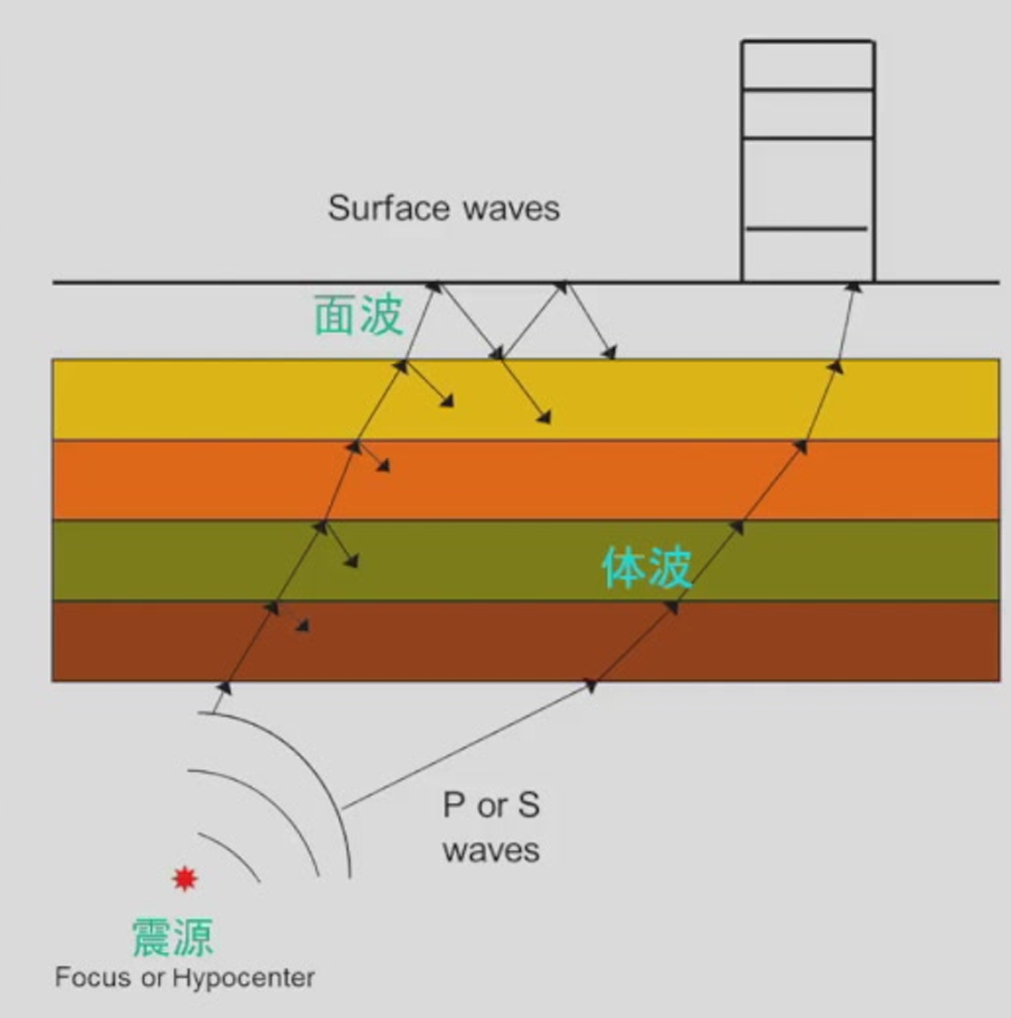
\includegraphics[width=0.5\textwidth]{../figure/dizhenbo.png}
    \caption{面波和体波}
\end{figure}

\begin{remark}
    一般认为,面波是体波经地层界面多次反射、折射所形成的次生波。

    如果把地球看作匀质球体,先到的波通常为纵波或P波;后到的波通常为横波或S波。

    纵波(P波):使建筑物产生上下颠簸

    横波(S波):使建筑物产生水平摇晃
\end{remark}

面波也有两种,一种为瑞雷波(R波),一种为洛夫波(L波)。

\begin{enumerate}
    \item 瑞雷波传播时,质点在与地面成垂直的平面内沿波的前进方向作椭圆运动。
    \item 洛夫波传播时,质点在地平面内作与波行进方向相垂直的振动。
\end{enumerate}

\begin{remark}
    地震地面运动的竖向运动由P波和R波引起(随堂小测)。
\end{remark}

\begin{table}[htbp]
    \centering
    \begin{tabular}{|>{\centering}m{3cm}|>{\centering}m{2cm}|>{\centering}m{2cm}|>{\centering\arraybackslash}m{3cm}|}
      \hline
      \multirow{2}{*}{\textbf{各种波特点}} 
        & \multicolumn{2}{c|}{\textbf{体波}} & \textbf{面波} \\ \cline{2-4}
      & \textbf{P波} & \textbf{S波}   & \textbf{R波和L波}     \\ \hline
      \textbf{波速}   & 快           & 较快           & 慢                     \\ \hline
      \textbf{周期}   & 短           & 较短           & 长                     \\ \hline
      \textbf{振幅}   & 小           & 较小           & 大                     \\ \hline
      \textbf{运动方向}
        & 上下运动
        & 前后、左右运动
        & R波:上下、前后运动;L波:左右运动 \\ \hline
    \end{tabular}
    \caption{各种波的特性比较}
  \end{table}

影响地面运动频谱的两个因素:
场地条件:(1)土层软硬程度(2)土层覆盖层厚度

震中距:周期短的波在有阻尼介质中传播较易衰减,随着震中距的增加,短周期成分占比减小,长周期成分占比增加
特定周期的波可能引发共振

\section{单质点体系运动方程}

\begin{definition}
    反应谱理论:
    $$F = k \beta G$$
\(G\) --- 重力荷载代表值;

\(k\) --- 地震系数(反映震级等的影响);

\(\beta\) --- 动力系数(反映结构的特性,如周期、阻尼等的影响)。

反应谱理论的成功之处在于,不仅考虑了地震的强度影响,还考虑了结构的抗震影响,但是没有考虑地震时间长度的影响。
\end{definition}

为分别考虑地面运动幅值和频谱对地震反应谱影响,将 \( F = m \cdot S_a \) 表达式改写为:

\[
F = m S_a = mg \left( \frac{\left| \ddot{x}_g \right|_{\text{max}}}{g} \right) \left( \frac{S_a}{\left| \ddot{x}_g \right|_{\text{max}}} \right) = G k \beta
\]
\[
S_a = \left| \ddot{x}_g + \ddot{x} \right|_{\text{max}}
\]
式中:\( k \) 为地震系数

\( \beta \) 为动力系数

\( G = mg \) 为结构重量

\(\left| \ddot{x}_g \right|_{\text{max}}\) 为地面运动最大加速度

\begin{remark}
    地震影响系数: $\alpha = k\beta$
\end{remark}

\begin{figure}[H]
    \centering
    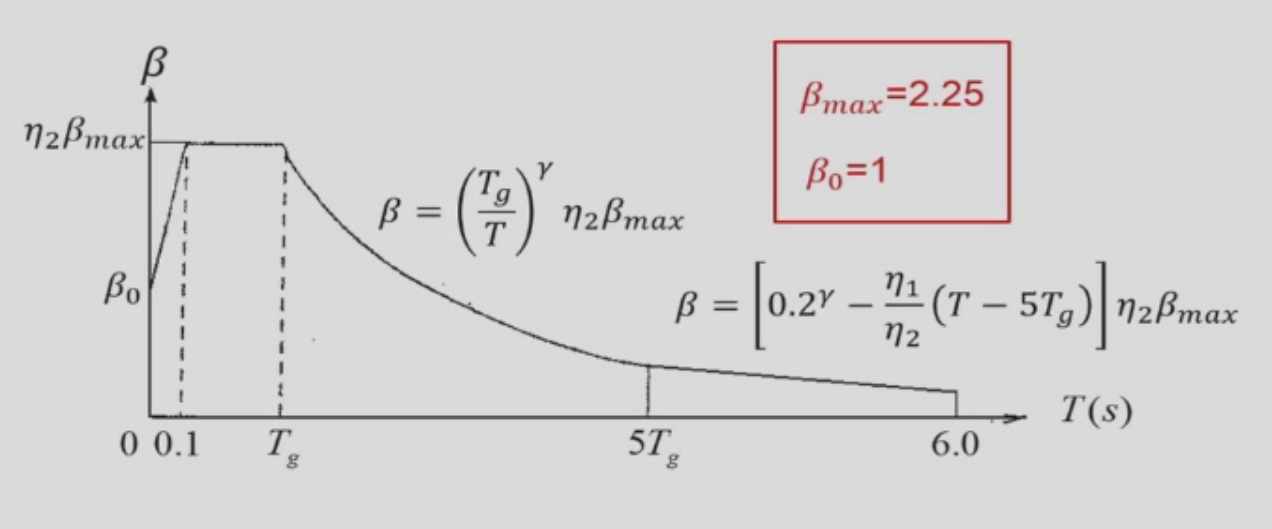
\includegraphics[width=0.8\textwidth]{../figure/beta.png}
    \caption{地震系数}
\end{figure}

\begin{figure}[H]
    \centering
    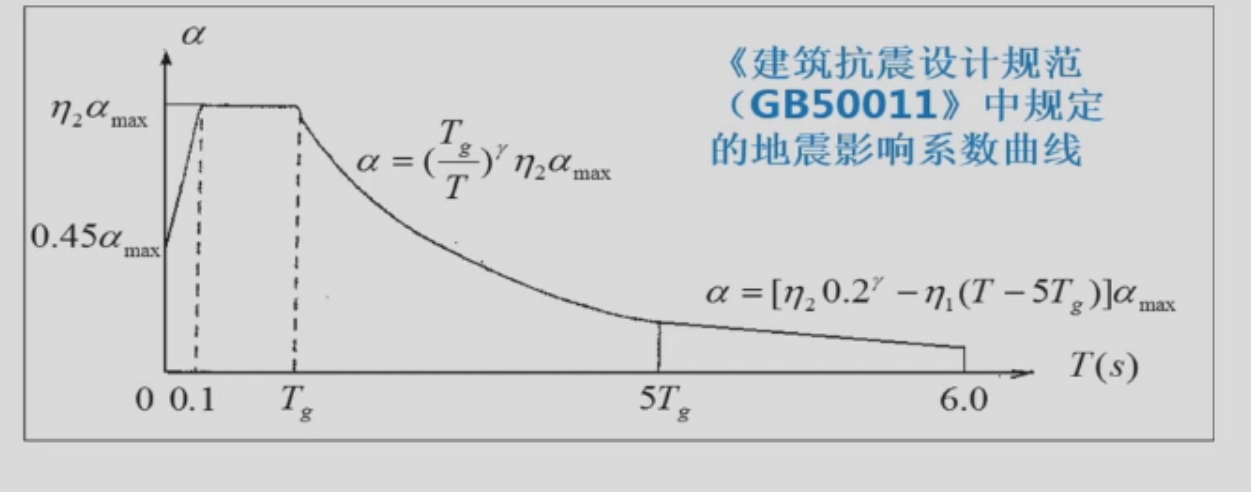
\includegraphics[width=0.8\textwidth]{../figure/alpha.png}
    \caption{地震影响系数}
\end{figure}

\begin{figure}[H]
    \centering
    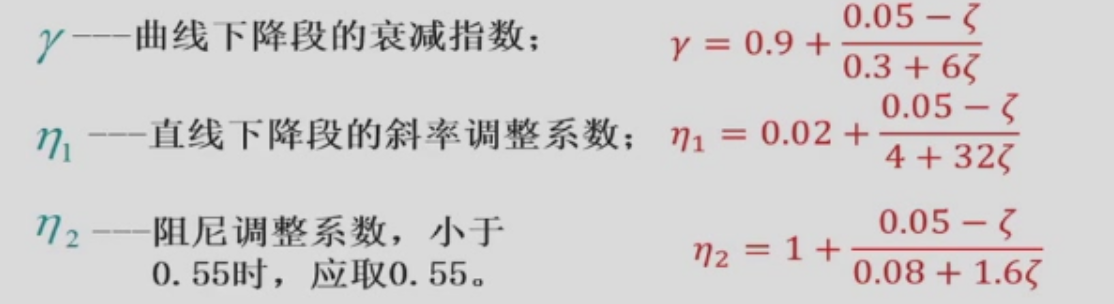
\includegraphics[width=0.8\textwidth]{../figure/canshu.png}
    \caption{相关参数}
\end{figure}

\begin{remark}
    知道了地震影响系数,根据两个图,可以分别计算出地震系数和动力系数,比如说曲线下降段的k=1。
\end{remark}

\begin{remark}
    地震作用是一种间接作用\&偶然作用\&动态作用
\end{remark}

\section{多质点体系运动方程}
当结构的质量不集中于一个确定位置时,如多高层房屋、烟囱等,应将结构处理成多质点体系进行地震反应分析,才能得到切合实际的解答。

\textbf{以下关于振型分解反应谱法的内容不是那么重要,沈老师强调了重点考虑底部剪力法}

通俗的理解下,振型分解反应谱法(因为我也看的不是很懂):

对于一个多质点体系,每个节点,都可以列一个和单质点体系类似的方程,简写为矩阵的形式:
\[[M] \{ \ddot{x} \} + [C] \{ \dot{x} \} + [K] \{ x \} = - \ddot{x}_g [M] \{ 1 \}\]
类似的写出特征方程:
\[([K] - \omega^2 [M]) \{\phi\} = 0\]
从线性代数角度来说,这个方程的特征向量线性无关,所以通解可以表示为特征向量的线性组合形式。
\[\mathbf{x}(t) = \sum_{r=1}^{n} \phi_r q_r(t)\]
这里的$q_r(t)$就是以振型为基底的新坐标(相当于线性变换了)
同时这里刚度矩阵$K$和$M$为对称矩阵,$\omega^2$也是对称矩阵,因此振型是相互正交的。
\begin{remark}
    对称矩阵的特征向量相互正交。

\end{remark}
同新坐标系下的$\mathbf{x}(t)$带入原方程,进行求解
\[
\ddot{q}_j + 2\omega_j \zeta_j \dot{q}_j + \omega_j^2 q_j = -\gamma_j \ddot{x}_g
\]
得到反应谱的定义:
$$F_{ji} = m_i \gamma_j \phi_{ji} S_a(T_j) = \gamma_j \phi_{ji} G_i \alpha(T_j)$$
考虑到各阶振型不在同一时刻发生,各振型最大效应直接相加结果会偏大,因此需要采取合理的振型组合,常用方法“平方和开方”法
$$S = \sqrt{\sum S_j^2}$$
S——水平地震作用效应;

$S_j$——j振型水平地震作用产生的作用效应,包括内力和变形。

一般,各阶振型在地震总效应中的贡献随其频率的增加而迅速减少,频率最低的几个振型控制着结构的最大地震效应。实际计算中,一般采用前几个振型即可。

\begin{figure}[H]
    \centering
    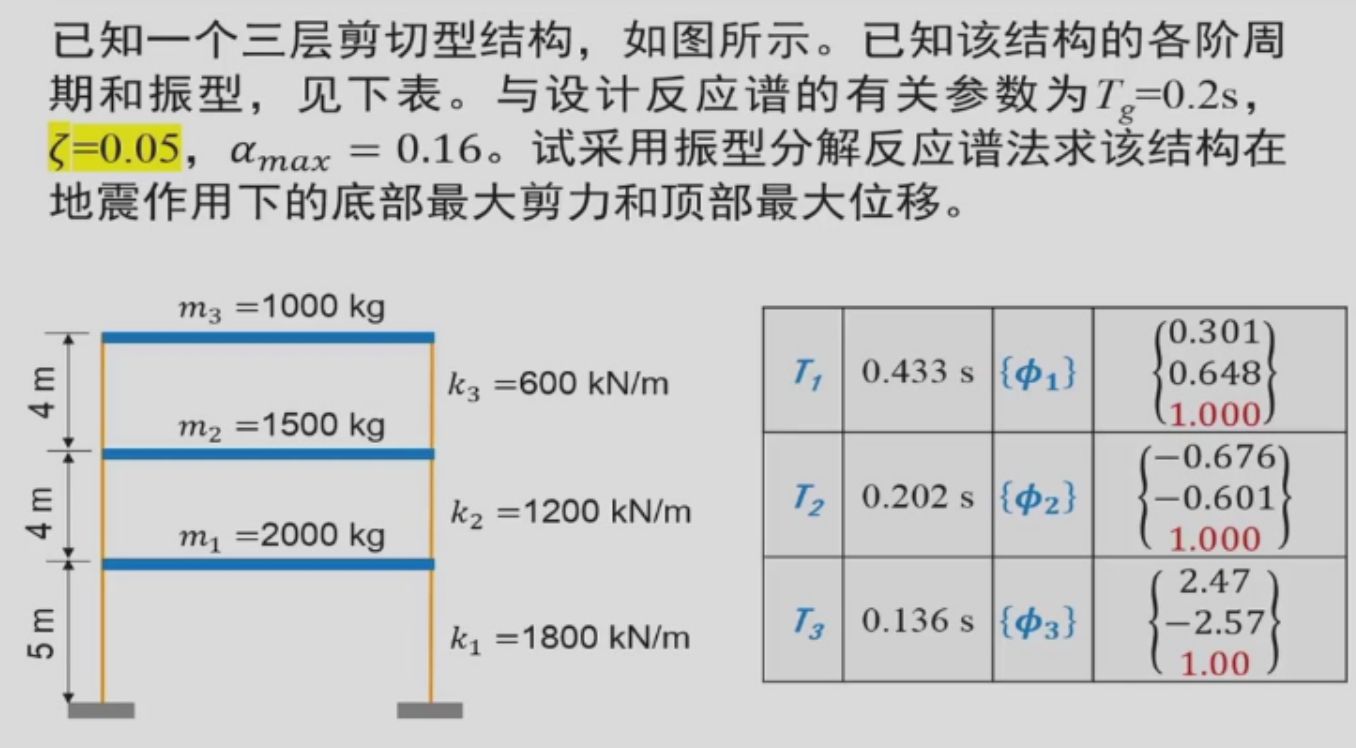
\includegraphics[width=0.8\textwidth]{../figure/zhengxingfenjie.png}
    \caption{振型分解计算例题}
\end{figure}

\begin{remark}
    \[
    \gamma_j = \frac{\{\phi_j\}^T [M] \{1\}}{\{\phi_j\}^T [M] \{\phi_j\}}
    \]
    \[
    F_{ij}=G_i\gamma_{i}\phi_{ij}\alpha_{i}
    \]
\end{remark}

\begin{figure}[H]
    \centering
    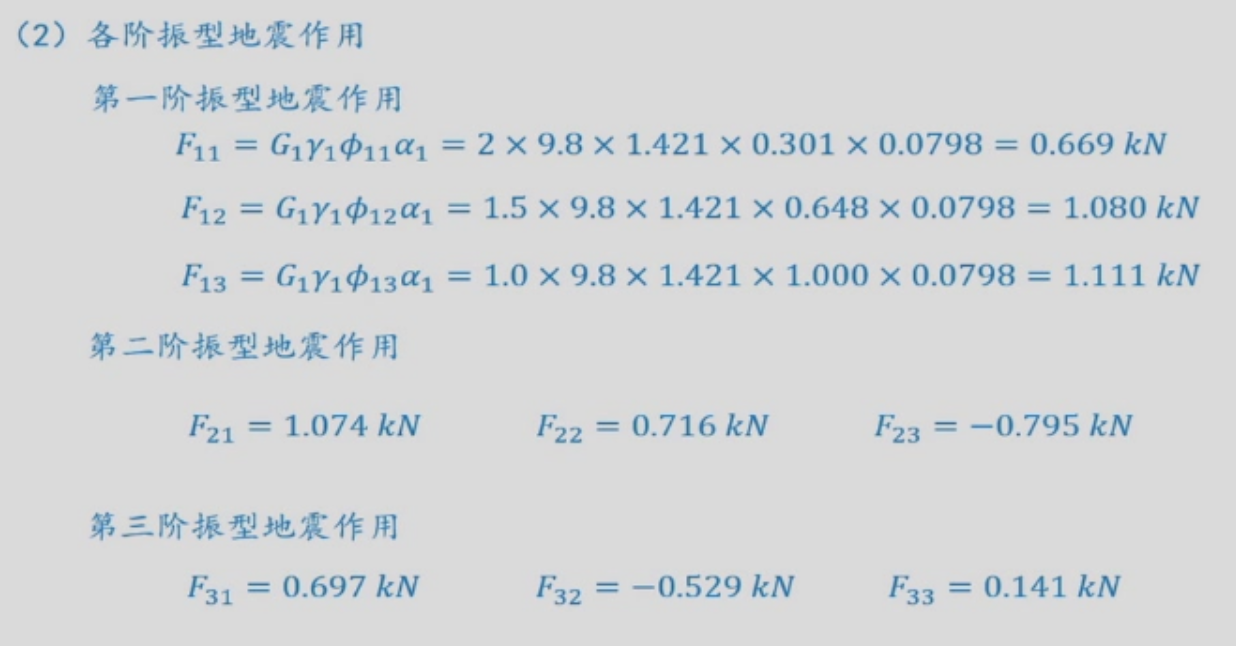
\includegraphics[width=0.8\textwidth]{../figure/ex1.png}
    \caption{计算作用力}
\end{figure}

\begin{figure}[H]
    \centering
    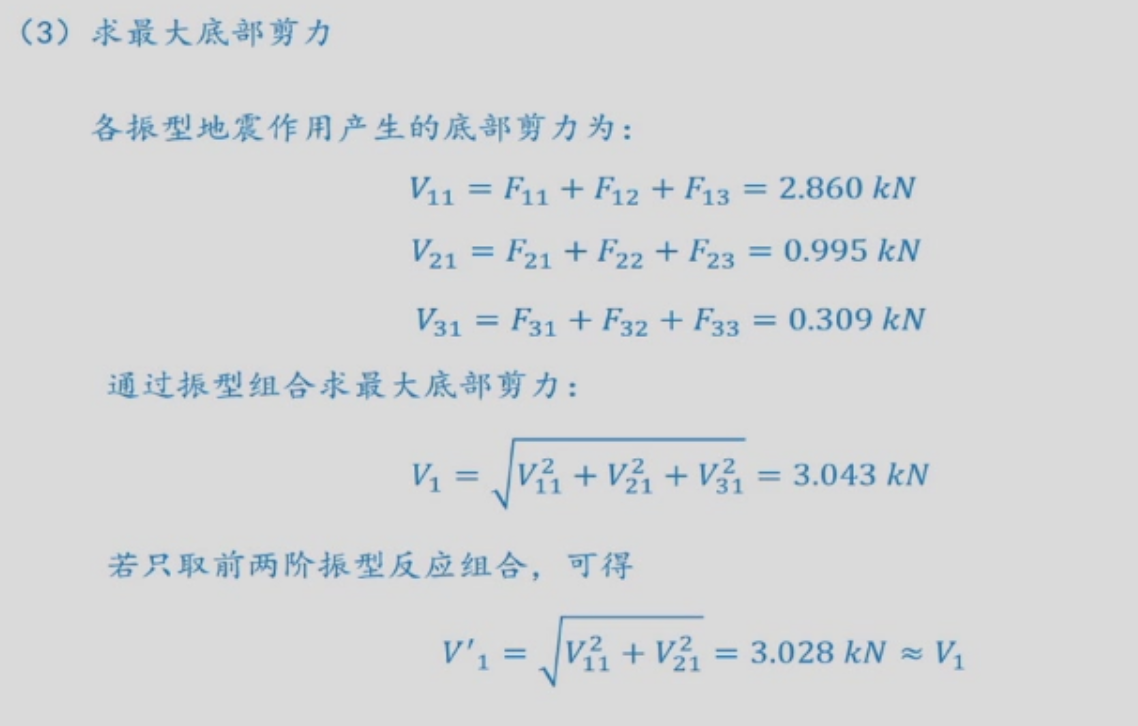
\includegraphics[width=0.8\textwidth]{../figure/ex2.png}
    \caption{计算剪力}
\end{figure}

\begin{figure}[H]
    \centering
    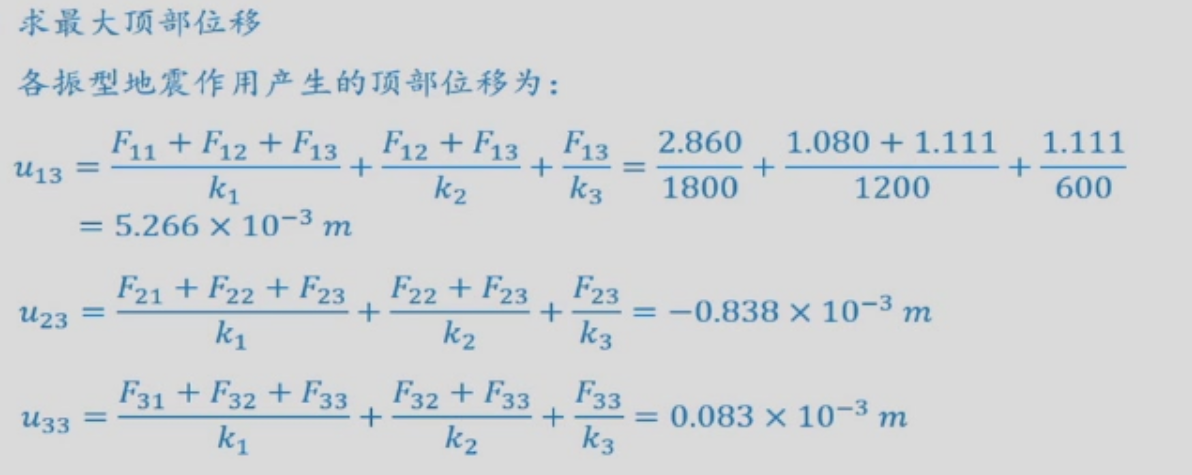
\includegraphics[width=0.8\textwidth]{../figure/ex3.png}
    \caption{计算位移}
\end{figure}

底部剪力法是把地震作用当作等效静力作用在结构上,以此计算结构的最大地震反应。因该方法首先计算地震产生的结构底部最大剪力,然后将该剪力分配到结构各质点上作为地震作用,而得此名。

\begin{remark}
    底部剪力法只考虑第一振型的地震作用,因此在计算时只需要计算体系的基本周期和第一振型。(×计算的时候不用第一振型只用基本周期)

    同时底部剪力法和振型分解反应谱法都是静力学方法,所以只适用弹性(非塑形)计算。
\end{remark}

\textbf{计算假定:}

\begin{enumerate}
    \item 地震作用下以第一振型反应为主,忽略其他振型反应

    \item 结构第一振型为线性倒三角形分布,任一质点的振型坐标与该质点离地面的分布假设高度成正比
\end{enumerate}

底部剪力法适用条件:

1. 房屋结构的质量和刚度沿高度分布比较均匀

2. 房屋高度不超过40m

3. 房屋结构在地震作用下的变形以剪切变形为主

4. 房屋结构在地震作用下的扭转效应可忽略不计

\begin{theorem}
    第一振型的水平地震作用为:
\[F_i = \alpha_1 \phi_{1i} \gamma_1 G_i = \alpha_1 \phi_{1i} \frac{\sum G_j \phi_{1j}}{\sum G_j \phi_{1j}^2} G_i\]
\[
\phi_{1i} = cH_i \quad \Longrightarrow
\]
\[
F_i = \alpha_1 \frac{\sum G_j H_j}{\sum G_j H_j^2} H_i G_i \quad \text{这条式子告诉我们}F_i\text{按}G_j H_j\text{分配}
\]
\[
F_i = \frac{G_i H_i}{\sum_{j=1}^{n} G_j H_j} F_{Ek}
\]
\[ F_{EK} = \alpha_1 \chi G_E \]
其中:
\[ \chi = \frac{(\sum G_j H_j)^2}{(\sum G_j H_j^2)(\sum G_i)} =\frac{3(n+1)}{2(2n+1)}\]
\[ G_E = \sum G_i \]

\end{theorem}

\begin{remark}
    $\gamma_j$被称为振型参与系数,表示各个振型被激发的"强度"。

    n=1,可以取$\chi$为1,大于1时,近似取为0.85
\end{remark}

\begin{remark}
    适用于基本周期:\( T_1 \leq 1.4T_g \)

当 \( T_1 > 1.4T_g \) 时,需考虑高振型的影响,否则计算所得的结构顶部地震作用偏小
\end{remark}

\begin{remark}
    \[\phi_{1i} = cH_i\]
    这条关系式的含义是由于第一振型是一个倒三角型,这在计算假定里
\end{remark}

\begin{figure}[H]
    \centering
    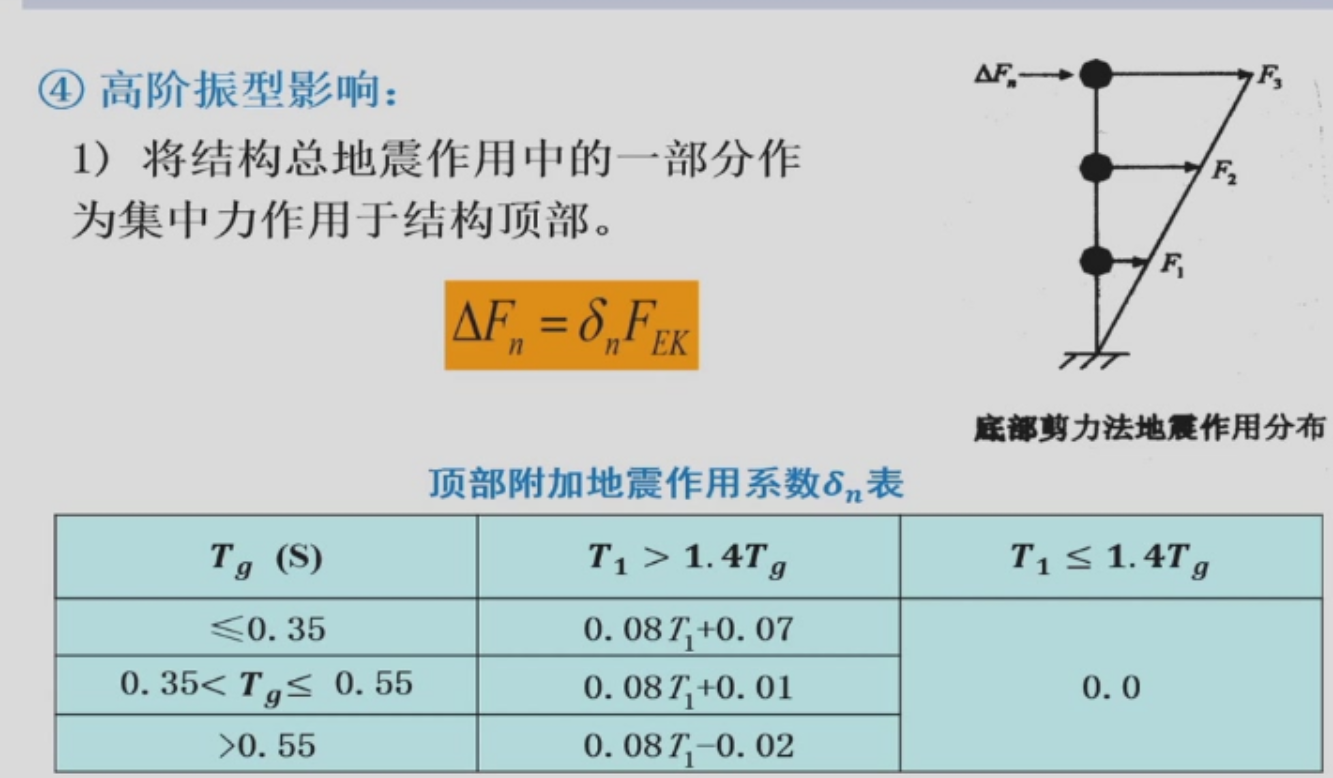
\includegraphics[width=0.8\textwidth]{../figure/gaojiezhengxing.png}
    \caption{高阶振型的影响}
\end{figure}

\begin{figure}[H]
    \centering
    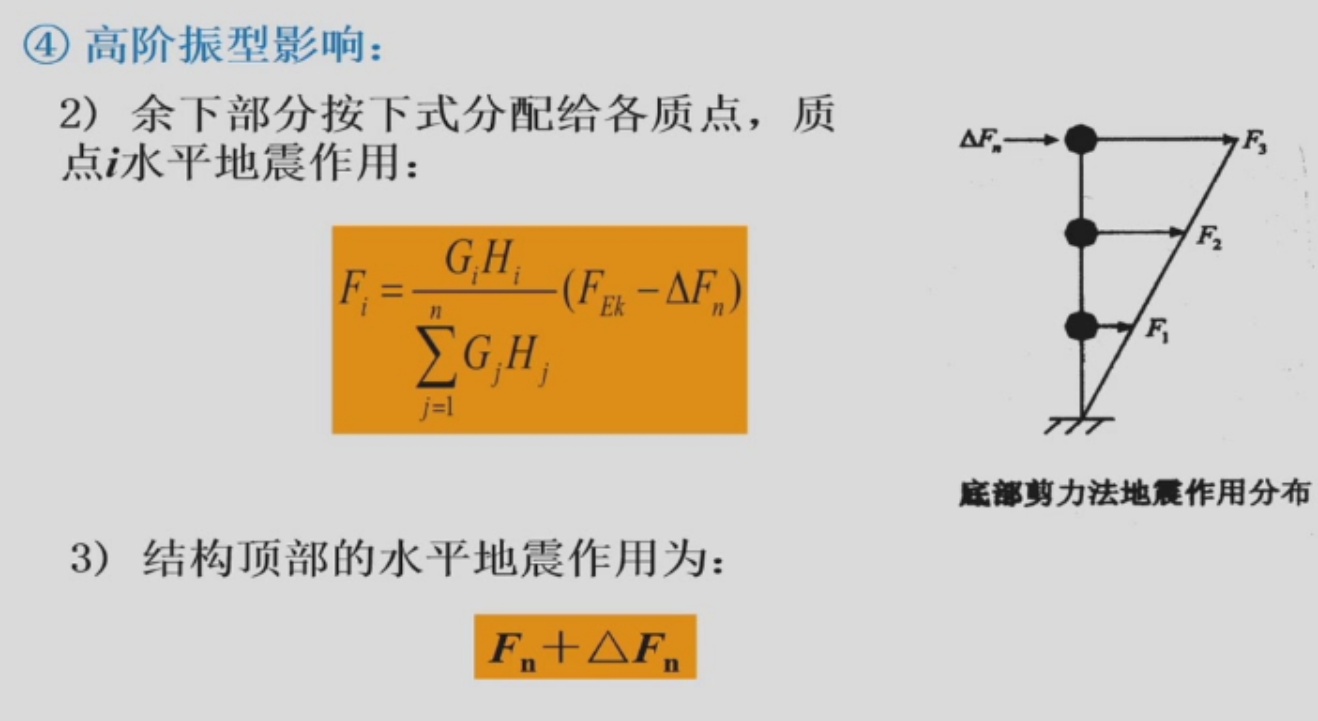
\includegraphics[width=0.8\textwidth]{../figure/gaojiezhengxing2.png}
    \caption{高阶振型对其余节点的影响}
\end{figure}

\begin{example}
    还是刚才那道题目

    求底部剪力

地震影响系数:\( \alpha_1 = \left( \frac{T_g}{T_1} \right)^{0.9} \quad \alpha_{\text{max}} = \left( \frac{0.2}{0.433} \right)^{0.9} \times 0.16 = 0.0798 \)

结构总重力荷载:\( G_E = (1.0 + 1.5 + 2.0) \times 9.8 = 44.1 \, kN \)

因结构质点数 \( n = 3 > 1 \),近似取 \( \chi = 0.85 \),则底部剪力:
\[ F_{E_k} = \chi \alpha_1 G_E = 0.85 \times 0.0798 \times 44.1 = 2.991 \, kN \]
与通过振型分解反应谱法求得的结果接近(3.043 kN)。

如不考虑高阶振型影响,则:
\[
F_1 = \frac{G_1 H_1}{\sum G_j H_j} F_{Ek} = \frac{2 \times 5}{2 \times 5 + 1.5 \times 9 + 1.0 \times 13} \times 2.991 = 0.819 \, kN
\]
\[
F_2 = \frac{1.5 \times 9}{2 \times 5 + 1.5 \times 9 + 1.0 \times 13} \times 2.991 = 1.106 \, kN
\]
\[
F_3 = \frac{1.0 \times 13}{2 \times 5 + 1.5 \times 9 + 1.0 \times 13} \times 2.991 = 1.065 \, kN
\]
顶部位移
\[
u_3 = \frac{F_{Ek}}{k_1} + \frac{F_2 + F_3}{k_2} + \frac{F_3}{k_3} = \frac{2.991}{1800} + \frac{1.065 + 1.106}{1200} + \frac{1.065}{600} = 5.246 \times 10^{-3} \, m
\]
与上例通过振型分解反应谱法求得的结果也很接近(5.333 $\times 10^{-3}$ m)。
\textbf{根据周期检查是否需要考虑高阶振型:}
\[ T_1 (= 0.433 \, s) > 1.4 T_g (= 0.28 \, s) \text{,需考虑高阶振型影响。} \]
查表:\[ \delta_n = 0.08 T_1 + 0.07 = 0.08 \times 0.433 + 0.07 = 0.105 \]
\[ \Delta F_3 = \delta_n F_{EK} = 0.105 \times 2.991 = 0.314 \, \text{kN} \]
则:
\[ F_1 = \frac{G_1 H_1}{\sum G_j H_j} (F_{Ek} - \Delta F_3) = \frac{2 \times 5}{2 \times 5 + 1.5 \times 9 + 1.0 \times 13} \times (2.991 - 0.314) = 0.733 \, \text{kN} \]
\[ F_2 = 0.990 \, \text{kN} \]
\[ F_3 = 0.953 \, \text{kN} \]
\[ F_3 + \Delta F_3 = 1.267 \, \text{kN} \]
顶部位移
\[ u_3 = \frac{F_{Ek}}{k_1} + \frac{F_2 + F_3 + \Delta F_3}{k_2} + \frac{F_3 + \Delta F_3}{k_3} = \frac{2.991}{1800} + \frac{2.257}{1200} + \frac{1.267}{600} \]
\[ = 5.654 \times 10^{-3} \, \text{m} \]
与通过振型分解反应谱法求得的结果接近(5.333 $\times 10^{-3}$ \text{m})。

\end{example}

\begin{remark}
    相比于原来反应谱方法,首先不论是剪力还是位移,都只要考虑一阶振型,简化了计算,同时精度在可控范围。
\end{remark}

\begin{example}
    简述地震反应谱的实质。

自振圆频率为 $\omega$,阻尼比为 $\xi$ 的单质点体系在确定的地震地面运动下最大的加速度反应。
\end{example}

\begin{example}
某三层钢筋混凝土框架结构,设计地震基本烈度为8度区,场地为Ⅳ类,设计地震分组为第二组,结构所在场地特征周期值 \(T_g = 0.75s\),结构层高和各层重力荷载代表值如图5-26所示,结构基本自振周期为0.50s。重力加速度 \(g = 9.8m/s^2\)。试采用底部剪力法,求:

(1) 结构的底部总剪力;

(2) 作用在各层楼板上的地震作用;

(3) 结构顶部最大位移。

\begin{figure}[H]
    \centering
    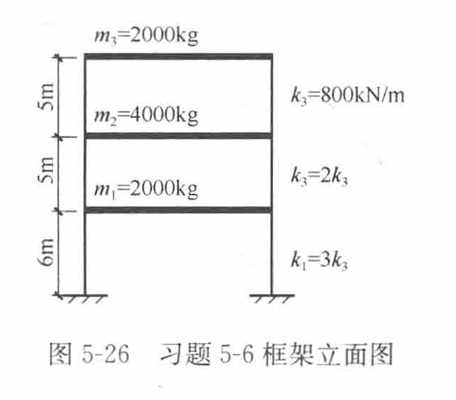
\includegraphics[width=0.6\textwidth]{../figure/4.png}
\end{figure}

    \[
    \delta_n = 0 \quad \text{查表可知,可以忽略地震的顶部作用。}
    \]
    \[
    (1)\quad F_{E_k} = a_{\max} \times \chi \times G = a_{\max} \times \chi \times \sum G_j = 0.16 \times 0.85 \times (2000 + 4000 + 2000) \times 9.8 = 10.66\,\text{kN}
    \]
    这里取$\chi = 0.85$,国家规范
    \[
    (2)\quad F_1 = \frac{6 \times 2}{6 \times 2 + 11 \times 4 + 16 \times 2} \times F_{E_k} = 1.45\,\text{kN}
    \]
    \[
    F_2 = 5.33\,\text{kN}
    \]
    \[
    F_3 = 3.87\,\text{kN}
    \]
    \[
    (3)\quad \sum U = U_1 + U_2 + U_3 = \frac{F_1 + F_2 + F_3}{k_1} + \frac{F_2 + F_3}{k_2} + \frac{F_3}{k_3} = 1.2 \times 10^{-2}\,\text{m}
    \]
\end{example}


\ifx\allfiles\undefined
\end{document}
\fi